%%%%%%%%%%%%%%%%%%%%%%%%%%%%%%%%%%%%%%%%%%%%%%%%%%%%%%%%%%%%%%%%%%%%%%%%%%%%%%%%
%                         FORMATO DE TESIS FI UNAM                             %
%%%%%%%%%%%%%%%%%%%%%%%%%%%%%%%%%%%%%%%%%%%%%%%%%%%%%%%%%%%%%%%%%%%%%%%%%%%%%%%%
% based on Harish Bhanderi's PhD/MPhil template, then Uni Cambridge
% http://www-h.eng.cam.ac.uk/help/tpl/textprocessing/ThesisStyle/
% corrected and extended in 2007 by Jakob Suckale, then MPI-iCBG PhD programme
% and made available through OpenWetWare.org - the free biology wiki

%                     Under GNU License v3

% ADAPTADO PARA FI-UNAM:  Jesús Velázquez y Marco Ruiz

\documentclass[twoside,11pt]{Latex/Classes/PhDthesisPSnPDF}
%         PUEDEN INCLUIR EN ESTE ESPACIO LOS PAQUETES EXTRA, O BIEN, EN EL ARCHIVO "PhDthesisPSnPDF.cls" EN "./Latex/Classes/"
\usepackage{blindtext}                        % Para insertar texto dummy, de ejemplo, pues.
% Note:
% The \blindtext or \Blindtext commands throughout this template generate dummy text
% to fill the template out. These commands should all be removed when 
% writing thesis content.
% This file contains macros that can be called up from connected TeX files
% It helps to summarise repeated code, e.g. figure insertion (see below).

%%%%%%%%%%%%%%%%%%%%%%%%%%%%%%%%%%%%%%%%%%%%%%
%            Colores de la UNAM              %
%%%%%%%%%%%%%%%%%%%%%%%%%%%%%%%%%%%%%%%%%%%%%%
%Azul Pantone 541  -->(0,63,119) RGB
\definecolor{Azul}{RGB}{0,63,119}

%Oro Pantone 460  -->(234,221,150) RGB
\definecolor{Oro}{RGB}{234,221,150}


%%%%%%%%%%%%%%%%%%%%%%%%%%%%%%%%%%%%%%%%%%%%%%
%            Comandos para líneas            %
%%%%%%%%%%%%%%%%%%%%%%%%%%%%%%%%%%%%%%%%%%%%%%
%Se define un comando \colorvrule para hacer líneas verticales de color con 3 argumentos: color, ancho, alto
\newcommand{\colorvrule}[3]{
\begingroup\color{#1}\vrule width#2 height#3
\endgroup}

%Se define un comando \colorhrule para hacer líneas horizontales de color con 2 argumentos: color, ancho
\newcommand{\colorhrule}[2]{
\begingroup\color{#1}\hrule height#2
\endgroup}

%%%%%%%%%%%%%%%%%%%%%%%%%%%%%%%%%%%%%%%%%%%%%%
%          Comando para derivadas            %
%%%%%%%%%%%%%%%%%%%%%%%%%%%%%%%%%%%%%%%%%%%%%%
\newcommand{\derivada}[3][]{\ensuremath{\dfrac{\mbox{d}^{#1}#2}{\mbox{d}#3^{#1}}}} 
%primer argumento(opcional): orden de la derivada
%segundo argumento: función a derivar
%tercer argumento: variable respecto a la que se deriva


%%%%%%%%%%%%%%%%%%%%%%%%%%%%%%%%%%%%%%%%%%%%%%
%       Comando para la exponencial          %
%%%%%%%%%%%%%%%%%%%%%%%%%%%%%%%%%%%%%%%%%%%%%%
\newcommand{\e}[1][]{\ensuremath{\mbox{e}^{#1}}}
%primer argumento(opcional): exponente de la exponencial




% insert a centered figure with caption and description
% parameters 1:filename, 2:title, 3:description and label
\newcommand{\figuremacro}[3]{
	\begin{figure}[htbp]
		\centering
		\includegraphics[width=1\textwidth]{#1}
		\caption[#2]{\textbf{#2} - #3}
		\label{condicion}
	\end{figure}
}

% insert a centered figure with caption and description AND WIDTH
% parameters 1:filename, 2:title, 3:description and label, 4: textwidth
% textwidth 1 means as text, 0.5 means half the width of the text
\newcommand{\figuremacroW}[4]{
	\begin{figure}[htbp]
		\centering
		\includegraphics[width=#4\textwidth]{#1}
		\caption[#2]{\textbf{#2} - #3}
		\label{#1}
	\end{figure}
}

% inserts a figure with wrapped around text; only suitable for NARROW figs
% o is for outside on a double paged document; others: l, r, i(inside)
% text and figure will each be half of the document width
% note: long captions often crash with adjacent content; take care
% in general: above 2 macro produce more reliable layout
\newcommand{\figuremacroN}[3]{
	\begin{wrapfigure}{o}{0.5\textwidth}
		\centering
		\includegraphics[width=0.48\textwidth]{#1}
		\caption[#2]{{\small\textbf{#2} - #3}}
		\label{#1}
	\end{wrapfigure}
}

% predefined commands by Harish
\newcommand{\PdfPsText}[2]{
  \ifpdf
     #1
  \else
     #2
  \fi
}

\newcommand{\IncludeGraphicsH}[3]{
  \PdfPsText{\includegraphics[height=#2]{#1}}{\includegraphics[bb = #3, height=#2]{#1}}
}

\newcommand{\IncludeGraphicsW}[3]{
  \PdfPsText{\includegraphics[width=#2]{#1}}{\includegraphics[bb = #3, width=#2]{#1}}
}

\newcommand{\InsertFig}[3]{
  \begin{figure}[!htbp]
    \begin{center}
      \leavevmode
      #1
      \caption{#2}
      \label{#3}
    \end{center}
  \end{figure}
}







%%% Local Variables:
%%% mode: latex
%%% TeX-master: "~/Documents/LaTeX/CUEDThesisPSnPDF/thesis"
%%% End:
           % Archivo con funciones útiles

%%%%%%%%%%%%%%%%%%%%%%%%%%%%%%%%%%%%%%%%%%%%%%%%%%%%%%%%%%%%%%%%%%%%%%%%%%%%%%%%
%                                   DATOS                                      %
%%%%%%%%%%%%%%%%%%%%%%%%%%%%%%%%%%%%%%%%%%%%%%%%%%%%%%%%%%%%%%%%%%%%%%%%%%%%%%%%
\title{Título de la tesis}
\author{Nombres Apellido1 Apellido2}        
\degree{Ingeniero en Carrera}               % Carrera
\director{Dr. Emmet L. Brown}               % Director de tesis
\degreedate{2112}                           % Año de la fecha del examen
\lugar{México, D.F.}                        % Lugar
%\portadafalse                              % Portada en NEGRO, descomentar y comentar la línea siguiente si se quiere utilizar
\portadatrue                                % Portada en COLOR

\keywords{tesis,autor,tutor,etc}            % Palablas clave para los metadatos del PDF
\subject{tema_1,tema_2}                     % Tema para metadatos del PDF  

%%%%%%%%%%%%%%%%%%%%%%%%%%%%%%%%%%%%%%%%%%%%%%%%%%%%%
%                   PORTADA                         %
%%%%%%%%%%%%%%%%%%%%%%%%%%%%%%%%%%%%%%%%%%%%%%%%%%%%%
\begin{document}

\maketitle									% Se redefinió este comando en el archivo de la clase para generar automáticamente la portada a partir de los datos

%%%%%%%%%%%%%%%%%%%%%%%%%%%%%%%%%%%%%%%%%%%%%%%%%%%%%
%                  PRÓLOGO                          %
%%%%%%%%%%%%%%%%%%%%%%%%%%%%%%%%%%%%%%%%%%%%%%%%%%%%%
\frontmatter
\begin{dedication}
A la Facultad de Ingeniería y a la  Universidad, por la formación que me han dado.\\
Es gracias a ustedes que es posible el presente trabajo.\\
En verdad, gracias.\\
Yo.
\end{dedication}
       % Comentar línea si no se usa
%\chapter*{}
%\pagenumbering{Roman}

\begin{acknowledgements}


  Sea éste trabajo un reconocimiento a mi familia; su esfuerzo, apoyo y amor 
  han sido componentes esenciales en mi vida.\\
  

  \noindent Un especial agradecimiento al Dr. Daniel Enrique Ceballos Herrera, su apoyo profesional
  para realizar éste trabajo es invaluable.\\

  \noindent A la memoria de mi padre, la mejor persona del mundo.

  \end{acknowledgements}




   % Comentar línea si no se usa 
% ******************************* Thesis Declaration ********************************

\begin{declaration}

Por la presente declaro que, salvo cuando se haga referencia específica al trabajo de otras personas, el contenido de esta tesis es original y no se ha presentado total o parcialmente para su consideración para cualquier otro título o grado en esta o cualquier otra Universidad. Esta tesis es resultado de mi propio trabajo y no incluye nada que sea el resultado de algún trabajo realizado en colaboración, salvo que se indique específicamente en el texto. 
% Author and date will be inserted automatically from thesis.tex


\end{declaration}
           % Comentar línea si no se usa

% Thesis Abstract -----------------------------------------------------


%\begin{abstractslong}    %uncommenting this line, gives a different abstract heading
\begin{abstracts}        %this creates the heading for the abstract page

    El presente trabajo se ocupa del diseño, análisis, desarrollo e implementación de un sistema transmisor óptico, desde la generación de una señal eléctrica hasta su adecuación al medio óptico.
    Los dispositivos y tecnologías empleadas, responden a la necesidad de generar un transmisor láser pulsado
    fácilmente reconfigurable, replicable y modular.

    Los transmisores láser, son un componente esencial en los sistemas de comunicación ópticos actuales dada su capacidad
    para transmitir grandes cantidades de información a grandes distancias, producto de sus bajas perdidas y su alta velocidad de transmisión.
    Por otra parte un transmisor láser, observado cómo sistema independiente encuentra aplicaciones diversas
    en sistemas de sensado y monitoreo.






    
    
%\blindtext

\end{abstracts}
%\end{abstractlongs}


% ----------------------------------------------------------------------                   % Comentar línea si no se usa

%%%%%%%%%%%%%%%%%%%%%%%%%%%%%%%%%%%%%%%%%%%%%%%%%%%%%
%                   ÍNDICES                         %
%%%%%%%%%%%%%%%%%%%%%%%%%%%%%%%%%%%%%%%%%%%%%%%%%%%%%
%Esta sección genera el índice
\setcounter{secnumdepth}{3} % organisational level that receives a numbers
\setcounter{tocdepth}{3}    % print table of contents for level 3
\tableofcontents            % Genera el índice 
%: ----------------------- list of figures/tables ------------------------
\listoffigures              % Genera el ínidce de figuras, comentar línea si no se usa
\listoftables               % Genera índice de tablas, comentar línea si no se usa


%%%%%%%%%%%%%%%%%%%%%%%%%%%%%%%%%%%%%%%%%%%%%%%%%%%%%
%                   CONTENIDO                       %
%%%%%%%%%%%%%%%%%%%%%%%%%%%%%%%%%%%%%%%%%%%%%%%%%%%%%
% the main text starts here with the introduction, 1st chapter,...
\mainmatter
\def\baselinestretch{1.5}                   % Interlineado de 1.5

% this file is called up by thesis.tex
% content in this file will be fed into the main document

%: ----------------------- HELP: latex document organisation
% the commands below help you to subdivide and organise your thesis
%    \chapter{}       = level 1, top level
%    \section{}       = level 2
%    \subsection{}    = level 3
%    \subsubsection{} = level 4

%----------------------- introduction file header -----------------------
%%%%%%%%%%%%%%%%%%%%%%%%%%%%%%%%%%%%%%%%%%%%%%%%%%%%%%%%%%%%%%%%%%%%%%%%%
%  Capítulo 1: Introducción- DEFINIR OBJETIVOS DE LA TESIS              %
%%%%%%%%%%%%%%%%%%%%%%%%%%%%%%%%%%%%%%%%%%%%%%%%%%%%%%%%%%%%%%%%%%%%%%%%%

\chapter{Introducción}

Los sistemas de comunicación óptica son una de las tecnologías más empleadas el sector de las telecomunicaciones en la actualidad; su desarrollo revolucionó la forma en que se transmite la información, mejorando de forma significativa la capacidad de canal, las velocidades de transmisión, las distancias alcanzadas así como la distancia entre dispositivos repetidores, parámetros que hasta 1970 se encontraban límitados por los principios de operación de los sistemas de microondas \citep{Agrawal2012}.

El uso de señales ópticas como portadoras en los sistemas de comunicación requiere de una fuente óptica coherente, un dispositivo detector y de un medio de transmisión adecuado; la invención del láser (por las siglas de \textit{Light amplification by stimulated  emission of radiation}) en 1960 \citep{Rawicz2008}, la investigación y desarrollo de fibras ópticas con perdidas menores a los 2 \si{\deci\belmilliwatt} en 1970 y de detectores de alta calidad en 1980 \citep{Tomasi2003} solventaron éstas necesidades dando paso al despliegue de sistemas de comunicación óptica confiables, de alta capacidad y económicamente viables. Estos sistemas fueron adoptados rápidamente, pues sus características permitieron abastecer la creciente demanda de servicios de comunicación y transferencia de información a través de las redes (Video, voz, comercio electrónico, educación a distancia, etc.), que en las décadas siguientes incrementarón no solo en calidad sino también en el ancho de banda necesario para su transmisión\citep{keiser3}.

La rápida adopción de los sistemas de comunicación óptica guiados por fibra óptica se debió también a sus notorias ventajas sobre los sistemas de comunicación tradicionales\footnote{Sistemas de comunicación que usan medios guíados convencionales de cable metálico \citep{Tomasi2003}}, entre las que encontramos expuestas por \citeauthor*{Tomasi2003} en \citep{Tomasi2003}: 

\begin{enumerate}
    \item Mayor capacidad de información: 
        Los cables metálicos generan capacitancia entre, e inductancia a lo largo, de sus conductores que los hacen funcionar como filtros pasabajas; eso limita sus frecuencias de transmisión y anchos de banda. Por otra parte, los sistemas de comunicación óptica tienen mayor capacidad de información debido a los anchos de banda inherentemente mayores a las frecuencias ópticas. 
    
    \item Inmunidad a la diafonía \footnote{La diafonía es el fenómeno que se presenta cuando se acoplan líneas conductoras paralelas y genera capacitancias parásitas que se manifiestan como interferencias en la comunicación.} e interferencia por estática: 
        Las fibras ópticas de vidrio o de plástico no son medios conductores de electricidad, por lo tanto no generan inducción magnética entre cables vecinos, haciéndolos medios inmunes a la diafonía \citep{nerivela}, por lo que además resultan inmunes a la interferencia electromagnética debida a rayos y otros dispositivos fuentes de ruido eléctrico. Por otra parte, las F.O. tampoco irradian energía de RF por lo que no representan fuentes de interferencia para otros sistemas de comunicaciones. 

    \item Durabilidad y seguridad: 
        Por la naturaleza del material de las F.O. , son mas resistentes ante ambientes adversos y cambios de temperatura; además de ser notablemente más ligeras que el cable metálico, pueden ser empleadas cerca de sustancias inflamables. Respecto a la seguridad e integridad de la información que viaja a través de la fibra, es virtualmente imposible intervenir una fibra óptica sin que el usuario o administrador lo sepa.
    
\end{enumerate}

Éstas características han permitido una notable penetración de los sistemas de comunicación óptica en todos los niveles estructurales de la redes de telecomunicaciones, desde los enlaces transoceanicos de gran capacidad hasta la implementación de FTTH como una tendencia cada vez mas adoptada.

Dada la gran cantidad de operaciones cotidianas en las que se involucran las tecnologías de comunicación óptica, resulta de vital importancia promover el desarrollo e investigación de metodologías novedosas que mejoren el desempeño de los dispositivos que constituyen a dichos sistemas; no solo aumento en la capacidad de transmisión, sino también en los métodos de monitoreo, resiliencia y adaptabilidad.


% pues resultan claras sus ventajas sobre las líneas de transmisión convencionales (Par de cobre, coaxial). Dada su continua aceptación y \cite{Shi2016} 

% dada su eficiencia, velocidad y demás ventajas provistas por éste desarrollo. Desde una visión esencialista, un sistema de comunicación óptico se compone por un transmisor, un medio de transmisión (Principalmente fibra óptica) y un receptor.
% La adecuación de señales eléctricas al medio óptico es en términos generales, la principal tarea ejecutada por un transmisor siguiendo el paradigma actual; además, éste principio no limita sus aplicaciones a un sistema de telecomunicaciones, sino también a sistemas de medición, reflectómetros y métodos de monitoreo y sensado.
    

%%%%%%%%%%%%%%%%%%%%%%%%%%%%%%%%%%%%%%%%%%%%%%%%%%%%%%%%%%%%%%%%%%%%%%%%%
%                           Presentación                                %
%%%%%%%%%%%%%%%%%%%%%%%%%%%%%%%%%%%%%%%%%%%%%%%%%%%%%%%%%%%%%%%%%%%%%%%%%

%\section{Presentación} % section headings are printed smaller than chapter names
%\blindtext

%%%%%%%%%%%%%%%%%%%%%%%%%%%%%%%%%%%%%%%%%%%%%%%%%%%%%%%%%%%%%%%%%%%%%%%%%
%                   Definición del problema                          %
%%%%%%%%%%%%%%%%%%%%%%%%%%%%%%%%%%%%%%%%%%%%%%%%%%%%%%%%%%%%%%%%%%%%%%%%%

\section{Definición del problema}

Las redes ópticas de telecomunicaciones emplean níveles ópticos en su operación y uno de los elementos más importantes involucrados en su desempeño es el sistema transmisor láser; sin embargo, estudiar su funcionamiento y arquitectura de forma experimental en los laboratorios de la Facultad de Ingeniería puede resultar prohibitivo dado el precio y complejidad de los dispositivos involucrados.

Una aproximación que permita manipular, editar y  actualizar la configuración de un sistema transmisor láser, tanto en el hardware como en el software, permitiría a los alumnos involucrarse de forma activa en su estudio y experimentación, así como habilitarlos para operar sistemas más complejos en el futuro.
%%%%%%%%%%%%%%%%%%%%%%%%%%%%%%%%%%%%%%%%%%%%%%%%%%%%%%%%%%%%%%%%%%%%%%%%%
%                   Hipótesis                                           %
%%%%%%%%%%%%%%%%%%%%%%%%%%%%%%%%%%%%%%%%%%%%%%%%%%%%%%%%%%%%%%%%%%%%%%%%%

\section{Hipótesis}

Es posible realizar la implementación de un transmisor láser pulsado desde la generación de pulsos con un microcontrolador, hasta su adecuación al medio óptico que pueda ser analizado de forma modular por los lectores del presente trabajo.
%%%%%%%%%%%%%%%%%%%%%%%%%%%%%%%%%%%%%%%%%%%%%%%%%%%%%%%%%%%%%%%%%%%%%%%%%
%                           Objetivo                                    %
%%%%%%%%%%%%%%%%%%%%%%%%%%%%%%%%%%%%%%%%%%%%%%%%%%%%%%%%%%%%%%%%%%%%%%%%%

\section{Objetivo}

Diseñar e implementar un transmisor láser pulsado que siente un antecedente académico en la Facultad de Ingeniería.

%%%%%%%%%%%%%%%%%%%%%%%%%%%%%%%%%%%%%%%%%%%%%%%%%%%%%%%%%%%%%%%%%%%%%%%%%
%                           Motivación y estado del arte                %
%%%%%%%%%%%%%%%%%%%%%%%%%%%%%%%%%%%%%%%%%%%%%%%%%%%%%%%%%%%%%%%%%%%%%%%%%
\section{Motivación y contribuciones}

Durante el estudio de los sistema de comunicaciones ópticas, resulta frecuente la aproximación exclusivamente analítica de los principios y dispositivos involucrados, mientras que la aproximación experimental se límita a la observación de los dispositivos en operación, la experimentación sobre configuraciones existentes y que a diferencia del estudio en sistemas electrónicos, dónde los componentes son reemplazables y configurables, la manipulación directa de los dispositivos láser y la arquitectura interna de los transmisores es más bien límitada. 

En la ésta tésis se presenta una propuesta de análisis, diseño e implementación de un sistema transmisor láser, de forma que resulte ilustrativa y representativa para explicar los elementos fundamentales de su operación. El diseño comprende un microcontrolador de la familia STM32 con arquitectura Arm, un sistema de control de corriente (Driver de corriente) basado en el amplificador operacional OPA 350 y un diodo láser comercial de 1550 nm.

%%%%%%%%%%%%%%%%%%%%%%%%%%%%%%%%%%%%%%%%%%%%%%%%%%%%%%%%%%%%%%%%%%%%%%%%%
%                           Estructura de la tesis                      %
%%%%%%%%%%%%%%%%%%%%%%%%%%%%%%%%%%%%%%%%%%%%%%%%%%%%%%%%%%%%%%%%%%%%%%%%%

\section{Estructura de la tesis}

Este trabajo está dividido en XX capítulos. En primera instancia se describen los principios teóricos que sustentan el desarrollo de cada elemento que compone al sistema transmisor, comenzando con los fundamentos de la arquitectura del microcontrolador para generar pulsos de corta duración, el método de operación del amplificador operacional como una fuente de corriente controlada y finalmente la naturaleza optoelectrónica del diodo láser. 
A continuación, en el capítulo 3, se describe de forma detallada el diseño y análisis llevado a cabo para conseguir el transmisor de pulsos con el desempeño deseado, así como las simulaciones requeridas y la estructura del código que ejecuta el microcontrolador. 

El capítulo 4 Resultados expone el desempeño logrado con el dispositivo implementado, las mediciones y la comparación con las estimaciones conseguidas mediante la simulación y la teoría previa. 

Finalmente, en el capítulo 5 revisamos las conclusiones a las que se llegarón tras el análisis de los resultados con la hipótesis inicial, además de hacer observaciones sobre las proyecciones del proyecto como un trabajo en continuo desarrollo, con aplicaciones en ejercicios que involucran transmisores láseres de pulsos.
            % ~10 páginas - Explicar el propósito de la tesis

%%%%%%%%%%%%%%%%%%%%%%%%%%%%%%%%%%%%%%%%%%%%%%%%%%%%%%%%%%%%%%%%%%%%%%%%%
%           Capítulo 2: MARCO TEÓRICO - REVISIÓN DE LITERATURA
%%%%%%%%%%%%%%%%%%%%%%%%%%%%%%%%%%%%%%%%%%%%%%%%%%%%%%%%%%%%%%%%%%%%%%%%%



\blindtext           % ~20 páginas - Poner un contexto a la tesis, hacer referencia a trabajos actuales en el tema

%%%%%%%%%%%%%%%%%%%%%%%%%%%%%%%%%%%%%%%%%%%%%%%%%%%%%%%%%%%%%%%%%%%%%%%%%
%           Capítulo 3: NOMBRE                   %
%%%%%%%%%%%%%%%%%%%%%%%%%%%%%%%%%%%%%%%%%%%%%%%%%%%%%%%%%%%%%%%%%%%%%%%%%

\chapter{Diseño e implementación}

En el presente capítulo se retoman los conceptos desarrollados en el capítulo anterior para describir el diseño e implementación del sistema transmisor láser empleando la tarjeta ede desarrollo STM32F446RE como generador de pulsos ópticos e interfaz de usuario, el amplificador operacional OPA350 cómo elemento principal del driver de corriente basado el diseño de la fuente de corriente Howland y finalmente se expone la operación y funcionamiento del diodo láser de 1550 nm como una fuente de pulsos ópticos modulados. 













% \chapter{Diseño del experimento}
% En este capítulo, se presenta la introducción al desarrollo de la tesis, ya sea el modelo matemático o las bases del proyecto, etc.
% Ejemplo de cita  [\citet{latex}]
% Ejemplo de cita [\citeauthor{RR73}]
 % The \cite command functions as follows:
 %   \citet{key} ==>>                Jones et al. (1990)
 %   \citet*{key} ==>>               Jones, Baker, and Smith (1990)
 %   \citep{key} ==>>                (Jones et al., 1990)
 %   \citep*{key} ==>>               (Jones, Baker, and Smith, 1990)
 %   \citep[chap. 2]{key} ==>>       (Jones et al., 1990, chap. 2)
 %   \citep[e.g.][]{key} ==>>        (e.g. Jones et al., 1990)
 %   \citep[e.g.][p. 32]{key} ==>>   (e.g. Jones et al., p. 32)
 %   \citeauthor{key} ==>>           Jones et al.
 %   \citeauthor*{key} ==>>          Jones, Baker, and Smith
 %   \citeyear{key} ==>>             1990





%%%%%%%%%%%%%%%%%%%%%%%%%%%%%%%%%%%%%%%%%%%%%%%%%%%%%%%%%%%%%%%%%%%%%%%%%
%                          Descripción de la planta                     %
%%%%%%%%%%%%%%%%%%%%%%%%%%%%%%%%%%%%%%%%%%%%%%%%%%%%%%%%%%%%%%%%%%%%%%%%%
% \section{Sección}
% El sistema blah, blah. Ejemplo de cita \citep{texbook}
% La figura (\ref{planta})                     %hace referencia a la imagen "planta" el número se inserta automáticamente
%  ilustra los componentes de la planta.

% \begin{figure}
%   \centering
%     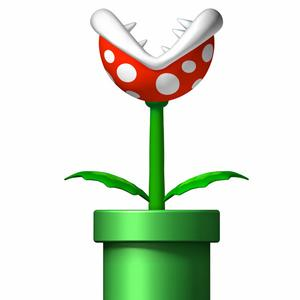
\includegraphics[scale=0.5]{Capitulo3/figs/planta.jpg}      %Ruta completa de la imagen, porque se compila desde el archivo tesis.tex
%   \caption{Descripción de la planta}            %Pie de imagen
%   \label{planta}                            %nombre de referencia
% \end{figure}




% %%%%%%%%%%%%%%%%%%%%%%%%%%%%%%%%%%%%%%%%%%%%%%%%%%%%%%%%%%%%%%%%%%%%%%%%%
% %                          Modelado                                     %
% %%%%%%%%%%%%%%%%%%%%%%%%%%%%%%%%%%%%%%%%%%%%%%%%%%%%%%%%%%%%%%%%%%%%%%%%%
% \section{\textcolor{Azul}{Sección en color azul}}
% \subsection{Subsección}
% Antes de comenzar, se definen  en la tabla ~\ref{tab:tabla} los parámetros y variables utilizadas

% %%%%%%%%Tabla Nombres de parámetros
% \begin{table}[ht]                             %Inicia el entorno table debajo del texto
% \centering\                                     %   centra la tabla
% \begin{tabular}{||c | c ||}                     %inicia entorno tabular con doble línea en las orillas, 2 columnas con el contenido centrado (c)
% \hline                                          %inserta línea horizontal
% \hline
% Nombre Parámetro/Variable & Símbolo\\
% \hline
% \hline
% Masa del péndulo & $m$ \\
% \hline
% Masa del carro & $M$\\
% \hline
% Distancia del eje de giro al centro de masa & $l$ \\
% \hline
% Aceleración gravitatoria & $g$ \\
% \hline
% Momento de inercia péndulo respecto del eje de giro& $J$ \\
% \hline
% Ángulo del péndulo respecto del eje vertical & $\theta$\\
% \hline
% Velocidad angular del péndulo & $\dot{\theta}$, $\omega$\\
% \hline
% Distancia del carro respecto al centro del riel & x\\
% \hline
% Velocidad del carro & $\dot{x}$, $v$\\
% \hline
% \hline
% \end{tabular}
% \caption[Parámetros dinámicos del carro-péndulo]{\textbf{Parámetros dinámicos del carro-péndulo} - Estos son los valores de parámetros utilizados en el diseño y las simulaciones, corresponden a los valores reales.}
% \label{tab:tabla}                              %etiqueta para referencia
% \end{table}

% \blindtext


% %%%%%%%%%%%%%%%%%%%%%%%%%%%%%%%%%%%%%%%%%%%%%%%%%%%%%%%%%%%%%%%%%%%%%%%%%
% %                          Subsección
% %%%%%%%%%%%%%%%%%%%%%%%%%%%%%%%%%%%%%%%%%%%%%%%%%%%%%%%%%%%%%%%%%%%%%%%%%

% \subsection{Otra subsección}

% \Blindtext      % ~20 páginas - Explicar el problema en específico que se va a resolver, la metodología y experimentos/métodos utilizados
\chapter{Análisis de Resultados}
\section{Resultados}
\Blindtext   % ~20 páginas - Presentar los resultados tal cual son, y analizarlos.
\chapter{Conclusiones}

Los sistemas de comunicación óptica son por 

\section{Verificación del a hipótesis}
            % ~5 páginas - Resumir lo que se hizo y lo que no y comentar trabajos futuros sobre el tema

%%%%%%%%%%%%%%%%%%%%%%%%%%%%%%%%%%%%%%%%%%%%%%%%%%%%%
%                   APÉNDICES                       %
%%%%%%%%%%%%%%%%%%%%%%%%%%%%%%%%%%%%%%%%%%%%%%%%%%%%%
\appendix
% this file is called up by thesis.tex
% content in this file will be fed into the main document
\chapter{Código/Manuales/Publicaciones}
% top level followed by section, subsection

\section{Apéndice}

Apéndice
               % Colocar los circuitos, manuales, código fuente, pruebas de teoremas, etc.

%%%%%%%%%%%%%%%%%%%%%%%%%%%%%%%%%%%%%%%%%%%%%%%%%%%%%
%                   REFERENCIAS                     %
%%%%%%%%%%%%%%%%%%%%%%%%%%%%%%%%%%%%%%%%%%%%%%%%%%%%%
% existen varios estilos de bilbiografía, pueden cambiarlos a placer
\bibliographystyle{apalike} % otros estilos pueden ser abbrv, acm, alpha, apalike, ieeetr, plain, siam, unsrt

%El formato trae otros estilos, o pueden agregar uno que les guste:
%\bibliographystyle{Latex/Classes/PhDbiblio-case} % title forced lower case
%\bibliographystyle{Latex/Classes/PhDbiblio-bold} % title as in bibtex but bold
%\bibliographystyle{Latex/Classes/PhDbiblio-url} % bold + www link if provided
%\bibliographystyle{Latex/Classes/jmb} % calls style file jmb.bst

\bibliography{Bibliografia/referencias}             % Archivo .bib


\end{document}